\newpage

\section{Attualizzazione dei rischi} \label{RiscontroRischi}

Vengono di seguito analizzati i problemi riscontrati durante lo svolgimento del progetto; ad ogni occorrenza rilevata corrisponderà poi una breve descrizione.\\

\subsection{Analisi dei requisiti}
\begin{table}[h!]
	\centerline{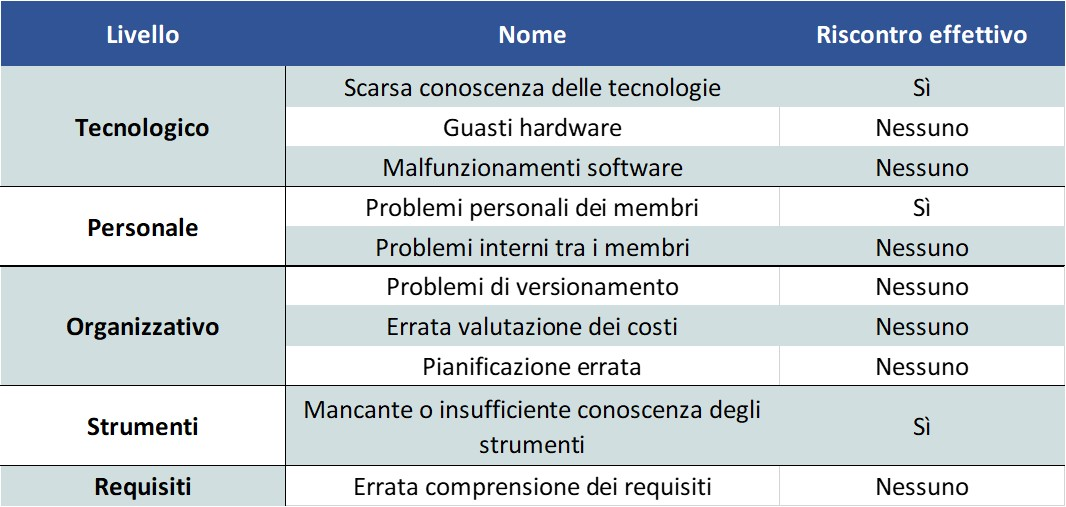
\includegraphics[scale=0.55]{img/RiscontroProblemi.jpg}}
	\caption{Resoconto dei problemi}
	\label{fig:resoconto_probl}
\end{table}

\subsubsection{Scarsa conoscenza delle tecnologie}
\paragraph {Descrizione}
Il gruppo era già conscio della mancanza di conoscenze delle tecnologie applicate; nonostante la fase iniziale, è stato necessario dedicare del tempo alla comprensione di alcune di queste, in particolare per quanto riguarda Ethereum e il funzionamento della blockchain in generale. Visto il rischio già preventivato, non ci sono stati particolari ritardi rispetto a quanto pianificato inizialmente.

\subsubsection{Problemi personali dei membri}
\paragraph {Descrizione}
\begin{itemize}
	\item Uno dei membri del gruppo è stato malato per una settimana; questo non ha causato particolari ritardi in quanto il tempo lavorativo è stato recuperato grazie agli slack time già preventivati per questi casi;
	\item Uno dei membri del gruppo è stato assente per alcuni giorni per impegni personali; l'assenza era stata comunicata con sufficiente anticipo per permetterne la corretta gestione.
\end{itemize}

\subsubsection{Pianificazione Errata}
\paragraph{Descrizione}
Ci sono stati dei ritardi sui tempi pianificati per la stesura delle \NdP{} dovuti all'inesperienza del gruppo. Tuttavia, questo non ha causato scostamenti della pianificazione generale per il primo periodo in quanto il ritardo è stato recuperato dal minor tempo necessario per la stesura dello \SdF{}. Questi due fattori hanno contribuito ad un impegno maggiore per gli \adms{}, mentre, in contrapposizione, ad un impegno minore per gli \anas{} in termini di tempo.

\subsubsection{Mancante o insufficiente conoscenza degli strumenti}
\paragraph {Descrizione}
Alcuni strumenti, essendo nuovi per la maggior parte dei membri, erano sconosciuti. Grazie allo studio individuale e all'aiuto degli \adms{}, è stato possibile colmare le lacune in tempi brevi e quindi non sono stati riscontrati ritardi rispetto a quanto pianificato inizialmente. Questo, però, ha contribuito ad un impegno maggiore in termini di tempo per gli \adms{}.